\documentclass{../bredelebeamer}
\usepackage{multirow}
\usepackage{pdfpages}
\usepackage{braket,bigstrut}
\usepackage{palatino}
\usepackage{multicol,bigstrut}
\usepackage{listings}
\usepackage{tikz}
\usepackage{pgfplots}
\pgfplotsset{compat=1.17}
\usepackage{booktabs}
\usepackage{amsmath,amssymb,amsfonts,cancel,physics,siunitx}
\usetikzlibrary{positioning,shadows,backgrounds,calc}%
\setbeamercolor{footnote mark}{fg=black}
\setbeamercolor{footnote}{fg=black}


\renewcommand{\baselinestretch}{0.9}

\usepackage[backend=bibtex8,style=authortitle,autocite=footnote]{biblatex}
%\addbibresource{../../references.bib}

\renewbibmacro*{cite:title}{%
	\printtext[bibhyperref]{%
		\printfield[citetitle]{labeltitle}%
		\setunit{\space}%
		\printtext[parens]{\printdate}%
	}%
}

\renewcommand{\figurename}{{\bf Fig.}}
\usefonttheme{serif} % default family is serif

\renewcommand{\baselinestretch}{0.9}

\title[]{Interference effects}
\subtitle{}
\author[Cristian F. Rodríguez]{
	$ $\\
	Cristian Fernando Rodríguez Cruz\\
	$ $\\
	$ $\\
	Authors:\\
	A. Flórez\inst{1}, \textcolor{Framableu}{\textbf{C. Rodriguez}}\inst{1}, J. Reyes-Vega\inst{1},\\
	J. Jones-Pérez\inst{2}. \\
    $ $\\
	$ $\\
}

\institute[Uniandes]{\inst{1} Universidad de los Andes\and
\inst{2} Pontificia Universidad Católica del Perú 
}
\date{\today}
\lstset{language=C++,
  basicstyle=\ttfamily,
  keywordstyle=\color{blue}\ttfamily,
  stringstyle=\color{red}\ttfamily,
  commentstyle=\color{green}\ttfamily,
  morecomment=[l][\color{magenta}]{\#}
}

\begin{document}
\frame{\titlepage}

\begin{frame}{Two body scattering}{CM-Frame}
    Consider the process
    \begin{equation}
        A(\va*{p}_1) + B(\va*{p}_2) \longrightarrow C(\va*{p}_3) + D(\va*{p}_4),
    \end{equation}
    \begin{center}
        \includegraphics[width=0.6\textwidth]{scatter.png}
    \end{center}

    From the Golden Rule, the cross section is given by
    \begin{equation}
        \sigma = \frac{S (2\pi)^4}{4\sqrt{(\va*{p}_1\cdot\va*{p}_2)^2 - (m_1m_2)^2}}\int \abs{\mathcal{M}}^2\delta^{(4)}(p_1 + p_2 - p_3 - p_4)\frac{d^3\va*{p}_3}{(2\pi)^3 2E_3}\frac{d^3\va*{p}_4}{(2\pi)^3 2E_4}.
    \end{equation}
    But, in the CM frame, $\va*{p}_1 + \va*{p}_2 = 0$, where
    \begin{gather}
        \sqrt{(\va*{p}_1\cdot\va*{p}_2)^2 - (m_1m_2)^2} = E_1E_2 \abs{\va*{p}_1},
        \\
        \delta^{(4)}(p_1 + p_2 - p_3 - p_4) = \delta\left(
        E_1 + E_2 - E_3 - E_4
        \right)
        \delta^{(3)}(\va*{p}_3 + \va*{p}_4).
    \end{gather}
    Thus
    \begin{equation}
        \sigma = \left(\frac{1}{8\pi}\right)^2 \frac{S}{(E_1E_2) \abs{\va*{p}_1}}\int \abs{\mathcal{M}}^2
        \frac{\delta\left(
            E_1 + E_2 - \sqrt{\va p_3^2 + m_3^2} - \sqrt{\va p_3^2 + m_4^2}
            \right)}{\sqrt{\va p_3^2 + m_3^2}\sqrt{\va p_3^2 + m_4^2}} \dd \va p_3
    \end{equation}
\end{frame}

\begin{frame}{Two body scattering}{CM-Frame}
    Integrating over the radial part $\abs{\va p_3}$, we get
    \begin{equation}
        \sigma = \left(\frac{1}{8\pi}\right)^2 \frac{S |\va*{p}_3|}{(E_1 +E_2)^2 \abs{\va*{p}_1}} \int \abs{\mathcal{M}}^2 \dd\Omega,
    \end{equation}
    with
    \begin{equation}
        |\va*{p}_3| = \frac{1}{2} \frac{\sqrt{((E_1+E_2)^2 - m_3^2 -m_4^2)^2- 4m^2_3m^2_4} }{E_1+E_2},
    \end{equation}
    the outgoing momentum in the CM frame.

    $$ $$

    We prefer work with differential cross section as
    \begin{equation}
        \frac{\dd \sigma}{\dd \Omega} = \frac{1}{64\pi^2} \frac{S }{(E_1 +E_2)^2 } \frac{|\va*{p}_3|}{\abs{\va*{p}_1}} \abs{\mathcal{M}}^2.
    \end{equation}


    Note that at this point, we don't need to know the explicit form of the matrix element $\mathcal{M}$, so it is a generic result.
\end{frame}

\begin{frame}{Two body scattering}{CM-Frame}
    Defining $\sqrt s = E_1 + E_2$, we have
    \begin{equation}
        |\va*{p}_3| = \frac{1}{2} \frac{\sqrt{(s - m_3^2 -m_4^2)^2- 4m^2_3m^2_4} }{\sqrt s}, \quad  |\va*{p}_1|=\frac{1}{2} \frac{\sqrt{(s - m_1^2 -m_2^2)^2- 4m^2_1m^2_2} }{\sqrt s}.
    \end{equation}
    so the differential cross section is
    \begin{equation}
        \frac{\dd \sigma}{\dd \Omega} = \frac{1}{64\pi^2} \frac{S }{s }
        \sqrt{\frac{(s - (m_3 + m_4)^2)(s - (m_3 - m_4)^2)}{(s - (m_1 + m_2)^2)(s - (m_1 - m_2)^2)}}
        \abs{\mathcal{M}}^2.
    \end{equation}

    In general, there are three Lorentz-invariant useful kinematical variables to describe the scattering process, known as Mandelstam variables:
    \begin{align}
        \hat s & = (p_1 + p_2)^2 = (p_3 + p_4)^2 = m_1^2 + m_2^2 + 2p_1^\mu p_{2\mu }= m_3^2 + m_4^2 + 2p_3^\mu p_{4\mu}, \\
        \hat t & = (p_1 - p_3)^2 = (p_2 - p_4)^2= m_1^2 + m_3^2 - 2p_1^\mu p_{3\mu }= m_2^2 + m_4^2 - 2p_2^\mu p_{4\mu},  \\
        \hat u & = (p_1 - p_4)^2 = (p_2 - p_3)^2= m_1^2 + m_4^2 - 2p_1^\mu p_{4\mu }= m_2^2 + m_3^2 - 2p_2^\mu p_{3\mu}.
    \end{align}
    In the CM-frame, $\hat s = s = (E_1+E_2)^2$.
\end{frame}

\begin{frame}{QED $e^+e^- \longrightarrow e^+e^-$ scattering}
    At tree level, there are two Feynman diagrams that contribute to the process
    \begin{minipage}{0.45\textwidth}
        \begin{center}
            \includegraphics[width=.6\textwidth]{../Images/Tchannel_ee_ee.png}
        \end{center}
        $$
            \left[\bar u_1'(ie\gamma^\mu) u_1\right]
            iD_{\mu\nu}(k_a)
            \left[\bar v_2(ie\gamma^\nu) v_2'\right]
        $$
        $$
            =-ie^2\frac{\left[ \bar u_1' \gamma^\mu u_1 \right]\left[ \bar v_2 \gamma_\mu v_2' \right]}{k_a^2}
        $$
        $$
            k_a = p_1 - p_1' = p_2' - p_2
        $$
    \end{minipage}\hfill
    \begin{minipage}{0.45\textwidth}
        \begin{center}
            \includegraphics[width=.6\textwidth]{../Images/Schannel_ee_ee.png}
        \end{center}
        \vspace{15pt}
        $$
            \left[\bar v_2(ie\gamma^\mu) u_1\right]
            iD_{\mu\nu}(k_b)
            \left[\bar u_1'(ie\gamma^\nu) v_2'\right]
        $$
        $$
            =-ie^2\frac{\left[ \bar v_2 \gamma^\mu u_1 \right]\left[ \bar u_1' \gamma_\mu v_2' \right]}{k_b^2}
        $$
        $$
            k_b = p_1 + p_2 = p_2' + p_1'
        $$
    \end{minipage}

    The fermionic exchange between the initial positron and the final electron is the same in both diagrams, so we have a relative minus sign between the two contributions.
    \begin{align}
        i\mathcal{M} & = ie^2 \left(
        \frac{
                \left[\bar u_1' \gamma^\mu u_1\right]\left[\bar v_2 \gamma_\mu v_2'\right]
            }{(p_1 - p_1')^2}
        -
        \frac{
                \left[\bar v_2 \gamma^\mu u_1\right]\left[\bar u_1' \gamma_\mu v_2'\right]
            }{(p_1 + p_2)^2}
        \right),
    \end{align}
\end{frame}
\begin{frame}{QED $e^+e^- \longrightarrow e^+e^-$ scattering}
    In terms of the Mandelstam variables, we have
    \begin{equation}
        i \mathcal{M}
        = ie^2 \left(
        \frac{
            \left[\bar u_1' \gamma^\mu u_1\right]\left[\bar v_2 \gamma_\mu v_2'\right]
        }{\hat t}
        -
        \frac{
            \left[\bar v_2 \gamma^\mu u_1\right]\left[\bar u_1' \gamma_\mu v_2'\right]
        }{\hat s}
        \right).
    \end{equation}
    So, the mean square of the matrix element is
    \begin{equation}
        \overline{|\mathcal{M}|^2} =\frac{1}{4}\sum_{\text{spins}} \abs{\mathcal M}^2= \frac{e^2}{4} \left(
        \frac{T_{11}}{\hat t^2}
        + \frac{T_{22}}{\hat s^2}
        - \frac{T_{12}+T_{21}}{\hat s\hat t}
        \right)
    \end{equation}
    with
    \begin{align}
        T_{11}            & = 32\left[ (\va{p}_1\cdot \va{p}_2)^2 + (\va{p}_1\cdot \va{p}_2')^2 + 2m^2(m^2 - \va{p}_1\cdot \va{p}_1') \right],
        \\
        T_{22}            & = 32\left[ (\va{p}_1\cdot \va{p}_1')^2 + (\va{p}_1\cdot \va{p}_2')^2 + 2m^2(m^2 + \va{p}_1\cdot \va{p}_2) \right],
        \\
        -T_{12} = -T_{21} & = 32 \left[
            (\va{p}_1\cdot \va{p}_2') +m^2\left(
            \va{p}_1\cdot \va{p}_2' + \va{p}_1\cdot \va{p}_2 - \va{p}_1\cdot \va{p}_1'
            \right)
            +m^4.
            \right]
    \end{align}
\end{frame}

\begin{frame}{Photon and $Z$-boson interference, $q \bar q \longrightarrow \tau^+ \tau^- $}
    
    \begin{minipage}{0.65\textwidth}
        The squared matrix element can be written as
        \begin{equation}
            \begin{aligned}
                \abs{\mathcal{M}}^2 & =\abs{\mathcal{M}_{\gamma^*}+\mathcal{M}_{Z}}
                \\&= \abs{\mathcal{M}_{\gamma^*}}^2 + \abs{\mathcal{M}_{Z}}^2 + 2\Re\left( \mathcal{M}_{\gamma^*}^*\mathcal{M}_{Z} \right).    \notag
            \end{aligned}
        \end{equation}
        In madgraph, with the sm model, we have
        \begin{itemize}
            \item \texttt{ q q$\sim$ $\rightarrow$ Z $\rightarrow$ ta+ ta-} for $\abs{\mathcal{M}_{Z}}^2$.
            \item \texttt{ q q$\sim$ $\rightarrow$ a $\rightarrow$ ta+ ta-} for $\abs{\mathcal{M}_{\gamma^*}}^2$.
            \item \texttt{ q q$\sim$ $\rightarrow$ ta+ ta- / h QED=2 } for $\abs{\mathcal{M}}^2$.
        \end{itemize}
    \end{minipage}
    \hfill
    \begin{minipage}{0.33\textwidth}
        \begin{center}
            \includegraphics[width=\linewidth]{../Images/DY.png}
        \end{center}
    \end{minipage}
    \pause
    $ $\\$ $\\$ $

    For the case $q_R \bar q_L \longrightarrow \tau_L^+ \tau_R^-$, the amplitudes are
    \begin{minipage}{0.65\textwidth}
        \begin{equation}
            \begin{aligned}
                \abs{\mathcal{M}_{\gamma^*}}^2          & = e^4\left[Q^{(f)} Q^{(q)}\right]^2\left[1+\cos \theta\right]^2                                                                      \\
                \abs{\mathcal{M}_{Z}}^2                 & = \frac{s^2 g_Z^4\left[g_R^{(f)} g_R^{(q)}\right]^2}{\textcolor{red}{\left(s-m_Z^2\right)^2+\left(m_Z \Gamma_Z\right)^2}}\left[1+\cos \theta\right]^2 \\
                \mathcal{M}_{\gamma^*}^*\mathcal{M}_{Z} & = \frac{g_Z^2 e^2 Q^{(f)} Q^{(q)} g_R^{(f)} g_R^{(q)}}{\textcolor{blue}{\left(s-m_Z^2+i \Gamma_Z\right)}} \textcolor{blue}{s}\left(1+\cos \theta\right)^2 \notag
            \end{aligned}
        \end{equation}
    \end{minipage}
    \hfill
    \begin{minipage}{0.33\textwidth}
        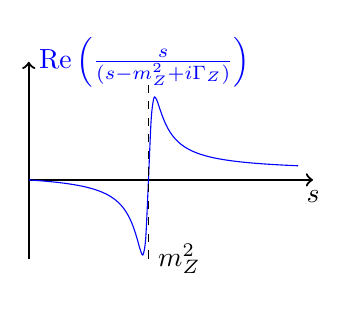
\begin{tikzpicture}[xscale=0.38, yscale=0.1]
            \draw[thick,->] (0,0) -- (9.5,0) node[below] {$s$};
            \draw[thick,->] (0,-10) -- (0,15) node[right,blue] {$ \Re\left(
                    \frac{s}{(s-m_Z^2+i \Gamma_Z)}
                    \right)$};

            % plot -(m^2 x)/((-m^2 + x)^2 + Γ^2) + x^2/((-m^2 + x)^2 + Γ^2), m=2, Γ=0.2
            \draw[domain=0:9,samples=100,smooth,variable=\x,blue]
            plot ({\x},{-(4*\x)/((4-\x)^2 + 0.04) + \x^2/((4-\x)^2 + 0.04)});
            % put a mark in s=m^2
            \draw[dashed] (4,-10) node[right] {$m_Z^2$} -- (4,12);
        \end{tikzpicture}
    \end{minipage}
\end{frame}

\begin{frame}{$gg (\rightarrow \Phi) \longrightarrow t\bar t$}{BSM scalar interference}
    The amplitude for the $gg (\rightarrow \Phi) \longrightarrow t\bar t$ process is
    \begin{equation}
        \mathcal{M}_{gg\rightarrow t \bar t}^\Phi = -\sum_\Phi \frac{\mathcal M_{gg\Phi} \hat s \mathcal M_{\Phi t\bar t}}{\hat s - m_\Phi^2 + i m_\Phi \Gamma_\Phi} + \mathcal M_{gg\rightarrow t\bar t}^\text{QCD}\;,
    \end{equation}
    And the BSM contributions $\frac{\mathrm{d} \hat{\sigma}_S}{\mathrm{~d} z}$, $\frac{\mathrm{d} \hat{\sigma}_I}{\mathrm{~d} z}$ to the QCD XS $\frac{\mathrm{d} \hat{\sigma}_B}{\mathrm{~d} z}$ are

    % \begin{minipage}{0.38\textwidth}
    %     The $A_{1/2}^{\Phi}$ is the helicity amplitude, gived by
    %     \begin{equation}\notag
    %         A_{1 / 2}^{H}\left(\tau_{t}\right)=2\left[\tau_{t}+\left(\tau_{t}-1\right) f\left(\tau_{t}\right)\right]
    %     \end{equation}
    %     if $\Phi$ is a scalar particle, or 
    %     \begin{equation}\notag
    %         A_{1 / 2}^{A}\left(\tau_{t}\right)=2\left[\tau_{t} f\left(\tau_{t}\right)\right]
    %     \end{equation}
    % \end{minipage}
    % \hfill
    % \begin{minipage}{0.60\textwidth}
        \begin{equation}
            \begin{aligned}
            \frac{\mathrm{d} \hat{\sigma}_S}{\mathrm{~d} z} & =\frac{3 \alpha_s^2 G_F^2 m_t^2}{8192 \pi^3} \hat{s}^2 \sum_{\Phi} \frac{\hat{\beta}_t^{p_\Phi}\left|\hat{g}_{\Phi t t}^2 A_{1 / 2}^{\Phi}\left(\tau_t\right)\right|^2}{\textcolor{red}{\left(s-M_{\Phi}^2\right)^2+\Gamma_{\Phi}^2 M_{\Phi}^2}} \\
            \frac{\mathrm{d} \hat{\sigma}_I}{\mathrm{~d} z} & 
            =-\frac{\alpha_s^2 G_F m_t^2}{64 \sqrt{2} \pi} \frac{1}{1-\hat{\beta}_t^2 z^2} \operatorname{Re}\left[\sum_{\Phi} \frac{\hat{\beta}_t^{p_{\Phi}} \hat{g}_{\Phi t t}^2 A_{1 / 2}^{\Phi}\left(\tau_t\right)}{\textcolor{blue}{s-M_{\Phi}^2+i \Gamma_{\Phi} M_{\Phi}}}\right]
            \end{aligned}\notag
        \end{equation}
        where $\hat{\beta}_t = \sqrt{1-4m_t^2/\hat{s}}$, $\tau_t = 4m_t^2/\hat{s}$, $z = \cos\theta$, and $p_\Phi \in \{3,1\}$.
    % \end{minipage}
    \begin{center}
        \includegraphics[width=0.9\textwidth]{../Images/gg_ttbar.png}
    \end{center}
\end{frame}

\begin{frame}{$gg (\rightarrow \Phi) \longrightarrow t\bar t$}{BSM scalar interference}
    \begin{center}
        \includegraphics[width=0.9\textwidth]{../Images/Interference_Scalars}
    \end{center}
\end{frame}

\begin{frame}{Interferences between the $Z'$ and the Vector Leptoquark}

    \begin{minipage}{.45\linewidth}
		\begin{center}
            \includegraphics[width=.62\linewidth]{../Images/non_resonant.png}
			\includegraphics[width=.6\linewidth]{../Images/Zp.png}
		\end{center}
		% \begin{equation*}
		% 	\mathrm{RKI}
        %     =\frac{1}{\sigma_{ LQ+Z'}}
        %     \dv{m}\left[
        %         \sigma_{ LQ+Z'}-\left(\sigma_{ LQ} +\sigma_{Z'}
        %         \vphantom{\frac{1}2}
        %         \right)
        %         \right]
		% \end{equation*}
	\end{minipage}	
	\begin{minipage}{.53\linewidth}
		The amplitudes has the form 
        \begin{align*}
            \mathcal{M}_{LQ} &\sim \frac{1}{t-m_{LQ}^2 + i m_{LQ} \Gamma_{LQ}},
        \end{align*}
        \begin{equation*}
            \mathcal{M}_{Z'} \sim \frac{1}{s-m_{Z'}^2 + i m_{Z'} \Gamma_{Z'}},
        \end{equation*}
        so the interference has the form
        \begin{equation}\notag
            \sim \frac{ m_{LQ}m_{Z'}\Gamma_{LQ}\Gamma_{Z'}- (t-m_{LQ}^2)(s-m_{Z'}^2)}{\left[
                (t-m_{LQ}^2)^2 + m_{LQ}^2\Gamma_{LQ}^2
            \right]
            \left[
                (s-m_{Z'}^2)^2 + m_{Z'}^2\Gamma_{Z'}^2
            \right]}.
        \end{equation}
	\end{minipage}
    with $t = (p_1 - p_3)^2 = (E_1 - E_3)^2 - (\va p_1 - \va p_3)^2$ and in CM frame, as $m_3=m_4$ and $m_1=m_2$ with $E_1=E_2=E_3=E_4=E$, we have
    \begin{equation}
        t = -\left(\va p_1 - \va p_3\right)^2 = - \va p_1^2 - \va p_3^2 + 2\va p_1\va p_3 
    \end{equation}
    where $\va p_1^2 = E^2 - m_b^2 $  and $\va p_3^2 = E^2 - m_\tau^2 $.
\end{frame}

\begin{frame}
    \begin{center}
        \includegraphics[width=0.95\textwidth]{../Images/interference_by_theta.pdf}    
    \end{center}
    
\end{frame}
\begin{frame}
    \begin{center}
        \includegraphics[width=0.95\textwidth]{../Images/interference_by_rel_width_Zp.pdf}
    \end{center}
\end{frame}

\begin{frame}{Interferences between the $Z'$ and the Vector Leptoquark}

    \begin{minipage}{.48\linewidth}
		\begin{center}
            \includegraphics[width=.62\linewidth]{../Images/non_resonant.png}
			\includegraphics[width=.6\linewidth]{../Images/Zp.png}
		\end{center}
		\begin{equation*}
			\mathrm{RKI}
            =\frac{1}{\sigma_{ LQ+Z'}}
            \dv{m}\left[
                \sigma_{ LQ+Z'}-(\sigma_{ LQ} +\sigma_{Z'}
                \vphantom{\frac{1}2}
                \right)
                \right]
		\end{equation*}
	\end{minipage}	
	\begin{minipage}{.50\linewidth}
		\includegraphics[width=.9\linewidth]{../Images/Kinematic_Interference_gu_1.0_gzp_1.0_zp_upper_limit_woRHC.pdf}
        $$ $$ 
        $$ $$
	\end{minipage}
	
\end{frame}

\end{document}